\section{Diseño de interiores}
\subsection{Definicion}
El diseño de interiores es una profesión en la cual soluciones creativas y técnicas son aplicadas dentro de una estructura para lograr la construcción de un entorno interno determinado. Éstas soluciones son funcionales, mejoran la calidad de vida de los ocupantes y son aestéticamente atractivas. Los diseños deben apegarse al código y normas requeridos, y fomentar los principios de sustentabilidad ambiental definidos por el edificio o empresa. El objetivo del diseño de interiores es lograr una armonía en los espacios que habitamos y dar confort al usuario de dichos espacios\cite{B01}. \par
El diseño de interiores sigue una metodología sistemática y coordinada que incluye investigación, análisis e integración de conocimientos dentro de un proceso creativo. Dentro ésta metodología podemos ubicar distintos servicios o etapas, dependiendo de la complejidad del trabajo, en las cuales encontramos: definición de los requerimientos funcionales para los espacios de las habitaciones, planeación de espacios interiores, realización de planos de construcción, definición de especificaciones de ubicación, colores y acabados en piso, paredes, materiales, equipo, mobiliario y muebles, administración de contratos de fabricación o instalación, etc.\par
En Estados Unidos el diseño de interiores es la única rama del diseño que está sujeta a las regulaciones federales y la ley gubernamental\cite{B02}.
\subsection{Movimientos en el diseño de interiores}

\subsubsection{Feng shui}
"El Feng Shui es un arte utilizado actualmente para alcanzar la armonización de las energías en las casas y los lugares de trabajo, basado en principios milenarios de la sabiduría china"\cite{B26}.Surge de la conjunción de dos ideogramas chinos que significan "viento" y "agua", dos conceptos que para las tradiciones de la antigüedad se relacionaban con el flujo y la circulación de la energía vita. Mediante este arte, nos es posible conocer cuál es la perfecta ubicación para edificar una casa, el lugar ideal para colocar cada uno de los muebles, como así también la forma de revertir las energías adversas que puedan afectarnos. El Feng Shui estudia la relación del hombre con la naturaleza y brinda la oportunidad de vivir de acuerdo con los principios que la rigen, y de esta manera, aprovechar esas energías que fluyen por todas partes y pueden influir en nuestro bienestar general.

\subsubsection{Deconstructivismo}
El desconstructivismo es la “Arquitectura que busca llegar a nuevas formas de expresión al alejarse de las restricciones estructurales y jerarquías funcionales y temáticas, enfocado 
hacia diseños a menudo no rectangulares, fantásticos y aparentemente inconexos”\cite{B24}. Tal trabajo a menudo representa una aplicación de las teorías filosóficas  de Jacques Derrida en Francia, que trato de llegar a nuevas ideas en la literatura; esta filosofía se ha aplicado desde finales del siglo 20 a las estructuras arquitectónicas generalmente llamadas arquitecturas deconstructivistas. \par
La arquitectura deconstructivista surge en una exposición, titulada deconstructivist architecture, que Philip Johnson y Mark Wigley organizaron en el museo de Arte Moderno (MoMa) de Nueva York en 1988.

\subsubsection{Diseño Orgánico}
Arquitectura cuyo diseño se establece de acuerdo con los procesos de la naturaleza en lugar de basarse en un diseño ya impuesto. Es una filosofía de diseño propuesta por Frank Lloyd Wright (1867-1959) a comienzos del siglo 20 y en ella afirma que un edificio (y su apariencia) deben de seguir formas que estén en armonía con su entorno natural.\cite{B24}\par  
Los materiales utilizados en el exterior deben ser acoplarse  con la ubicación del edificio, relacionando así el edificio a su entorno. Por lo tanto, debe hacerse de baja altura, con techos que sobresalgan para proporcionar protección del sol en el verano y para proporcionar alguna protección contra la intemperie en invierno además se debe de hacer un máxima uso de la luz natural.

\subsection{Fundamentos del diseño de interiores}
El diseño de interiores se ve como una actividad que tiene un punto de inicio (cuando el diseñador y el cliente tienen el primer contacto) y otro al final cuando el proyecto se ha ejecutado.\par
Se debe tomar en cuenta que el diseño de interiores es maleable, es decir, que su realización no está sujeto estrictamente a una serie de reglas. En un caso se puede realizar un determinado proceso, y en otro se puede realizar otro proceso diferente. No existe una solución estandarizada para para todos los casos.\par
Lo más importante es definir el por qué estamos diseñando. Por ejemplo si se está diseñando un armario, se tiene qué saber cuál es el impulso para hacerlo. El diseñador se plantea algunas ideas sobre las funciones que tiene un armario, el uso de la madera, reciclada, el del plástico o el nuevo material, y con base a eso, define el objetivo de diseñar el armario.
Otro fundamento importante es la armonía que se busca. Un espacio interior no sólo debe verse bonito, y tener colores agradables a la vista. Cada elemento que compone un espacio debe relacionarse con los demás. Un sillón en una sala de espera debe relacionarse y tener alguna conexión con la mesa de centro. Esta relación puede ser la similitud del acabado de ambos, la ubicación de uno con respecto al otro, etc.
Una habitación debe seguir un esquema de colores bien definido. Dentro de estos esquemas tenemos el monocromático, complementario y análogo, y cada uno deriva del círculo cromático.\par

\textbf{Monocromático}.- Es una selección de colores que funcionen bien juntos. Esto es trabajar con un matiz, y la variación de tintes, tonos, y sombras.
\begin{figure}[h!]
	\centering
	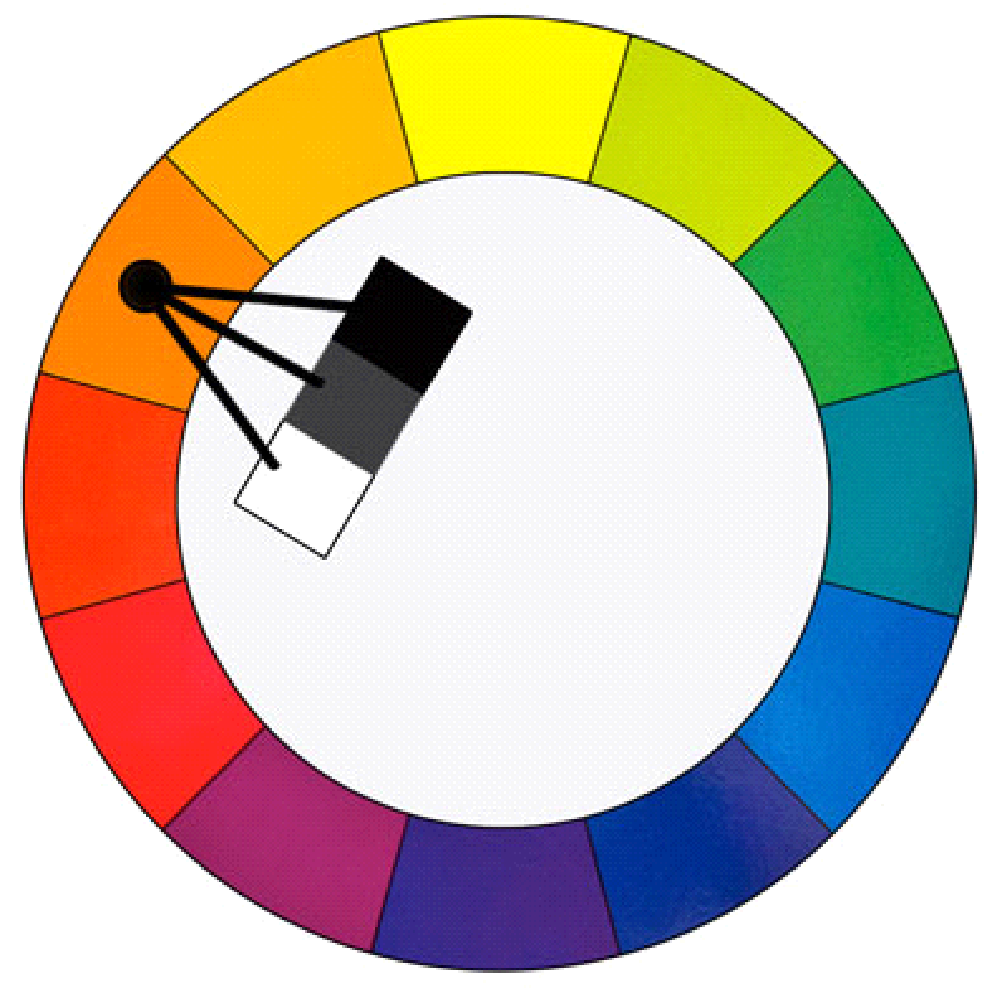
\includegraphics[width=7cm]{imagenes/marcoteorico/disenointeriores/monocromatico.png}
	\caption{Esquema monocromático.\cite{B13}}
	\label{fig:monocromatico}
\end{figure}

\textbf{Complementario}.- Los colores que se encuentran en extremos opuestos del círculo cromático se consideran complementarios. Al combinar estos dos colores, se puede expresar contraste e interés. Son difíciles de usar en grandes cantidades, pero por su contraste son muy buenos para resaltar algo, como un llamado de atención.
\begin{figure}[h!]
	\centering
	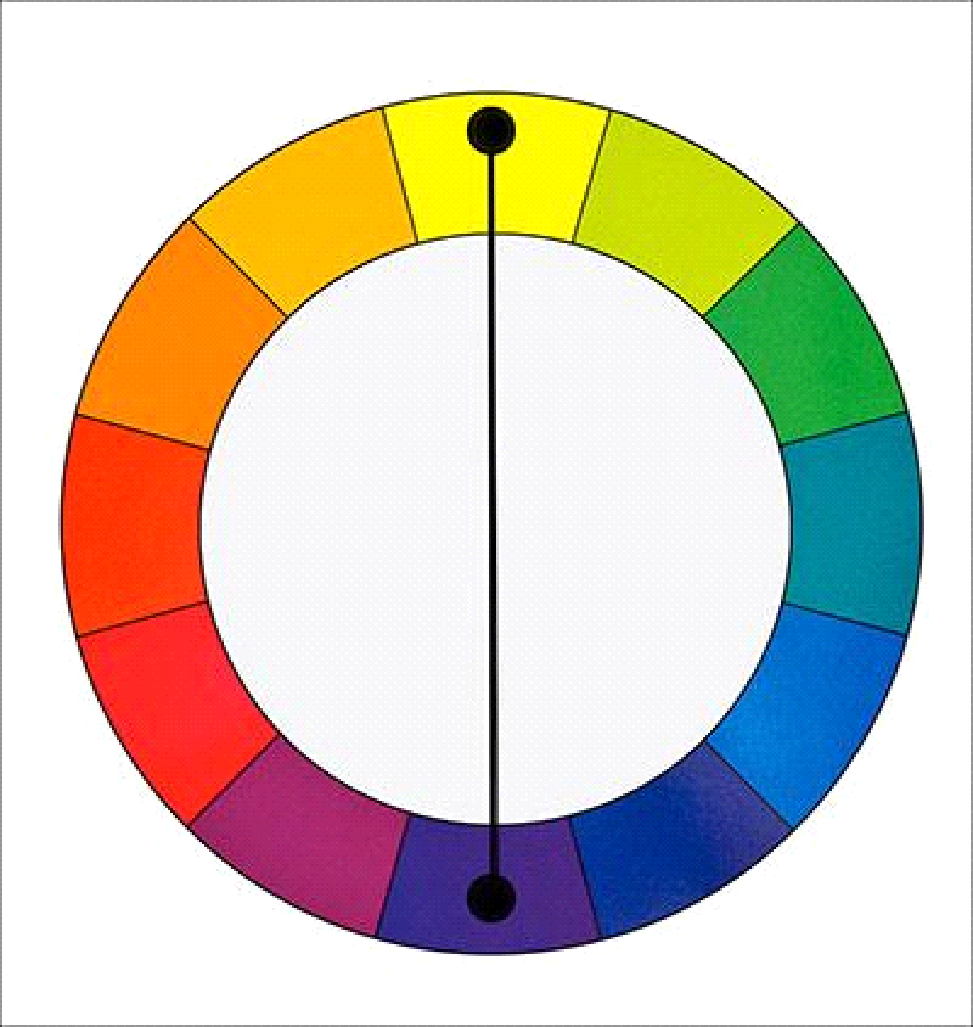
\includegraphics[width=7cm]{imagenes/marcoteorico/disenointeriores/complementario.png}
	\caption{Esquema complementario.\cite{B13}}
	\label{fig:complementario}
\end{figure}

\textbf{Análogo}.- Los colores que se encuentran al lado en el círculo cromático, son agradables juntos. Son la combinación perfecta, ya que son perfectos para cualquier uso, incluso para resaltar y contrastar un elemento específico sin demasiada interrupción. Como regla general, se debe seleccionar un color dominante, un segundo color para sustentar, y un tercer color para acentuar.\cite{B13}
\begin{figure}[h!]
	\centering
	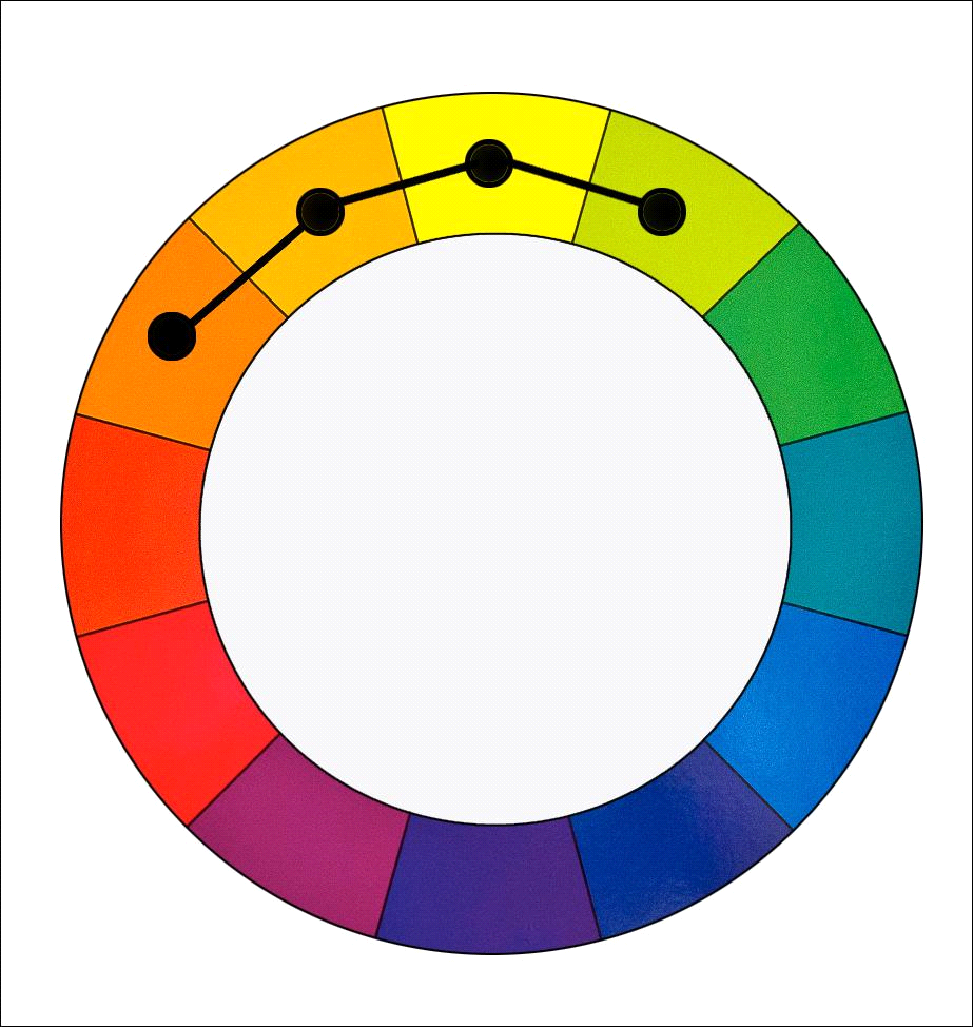
\includegraphics[width=7cm]{imagenes/marcoteorico/disenointeriores/analogo.png}
	\caption{Esquema análogo.\cite{B13}}
	\label{fig:analogo}
\end{figure}


\par 
